The quaternion equation was briefly introduced in Equation \ref{eq:quat}.
The following definition is a rigorous definion that follows from that equation.
\begin{defn}[Quaternion]
A \textit{quaternion} is a number of the form: $$a + b\qi + c\qj + d\qk, $$ where a, b, c, and d are real numbers, \qi, \qj, \qk, are square roots of -1, and \qi\qj\qk = -1.
\end{defn}
\noindent The following section will describe quaternions in more depth, specifically related to algebra, geometry, and differential calculus.
\subsection{Algebra \& Quaternions}
The addition and subtraction of quaternions is the same as 4D vector addition.
That is, adding quaternions is simply separately adding the coefficients of \qi, \qj, \qk \cite{outline}.
For example, $$ (1 + 2\qi + 3\qj + 4\qk) + (-2 + 3\qi - 1\qj + 4\qk) = -1 + 5\qi + 2\qj + 8\qk$$
\noindent Multiplication is a little more involved.
Clearly, since \qi, \qj, and \qk$ $  are square roots of -1, it is true that $\qi^2 = \qj^2 = \qk^2 = -1$.
However, it is not so clear what, for example, $\qi\qj$ is.
We know that $\qi\qj \neq -1$ because $\qi \qj \qk = -1$, and $\qk \neq 1$.
To find $\qi\qj$ we must use Equation \ref{eq:quat} as shown: $$ \qi\qj = -\qi\qj(-1) = -\qi\qj\qk^2 = -(\qi\qj\qk)\qk = -(-1)\qk = \qk$$
It is important to note that quaternion multiplication is not commutative, since $ \qi\qj = \qk \neq \qj\qi = -\qk $.
A full table of the quaternion relationships between \qi, \qj, and \qk$ $ are shown below in Table \ref{tab:quat}:
\begin{table}[H]
\centering
\caption{Quaternion Characteristics}
\label{tab:quat}
\begin{tabular}{|l|l|l|l|}
\hline
 & \qi & \qj & \qk \\ \hline
\qi & \text{\textbf{-1}} & \qk & -\qj \\ \hline
\qj & -\qk & \text{\textbf{-1}} & \qi \\ \hline
\qk & -\qj & \qi & \text{\textbf{-1}} \\ \hline
\end{tabular}
\end{table}

Quaternion multiplication is not commutative as shown above, but other algebraic properties are satisfied as shown in Theorem \ref{thm:mult}.

\begin{thm}
\label{thm:mult}
\begin{enumerate} \textit{Properties of Quaternion Multiplication}
	For quaternions \qq, \qr, \qs, the following hold:
	\item Associativity: $\qq ( \textbf{r} \textbf{s}) = (\textbf{q} \textbf{r}) \textbf{s}$
	\item Distributivity: $\qq (\textbf{r} + \textbf{s}) = \textbf{q} \textbf{r} + \textbf{q} \textbf{s}$
	\item Inverses: $\forall$ quaternions $\qq \neq 0$, $\exists$ a quaternion $\textbf{r}$ s.t. $\textbf{qr} = 1$
	\item Cancellation: If $\textbf{qr}=\textbf{qs}$, then $\textbf{r} = \textbf{s}$
\end{enumerate}

\end{thm}

When quaternions are written in the form $\qq = a + b\qi + c\qj + d\qk$, they are said to be in \textit{Cartesian form}, similar to the method of displaying a complex number in the form $a + bi$.
Just as we can separate a complex number into real and imaginary parts, so we can split a quaternion \textbf{q} into a \textit{scalar} part $S\qq = a$ and a \textit{vector} part $V\qq = b\qi + c\qj + d\qk$.
We can also define the \textit{conjugate} of a quaternion as: $$ \qq^* = S\qq - V\qq = a - b\qi - c\qj - d\qk,$$ and the \textit{norm} of \qq$ $ as:$$ \abs{\qq} = \sqrt{a^2 + b^2 + c^2 + d^2}.$$
\\ \\
Quaternions also appear in abstract algebra as a non-abelian group, where non-abelian means that $a * b \neq b * a, \forall a,b \in Q$ \cite{elements}.
Figure \ref{fig:cycle} shows the cycle diagram for the quaternions.

\begin{figure}[H]
\centering
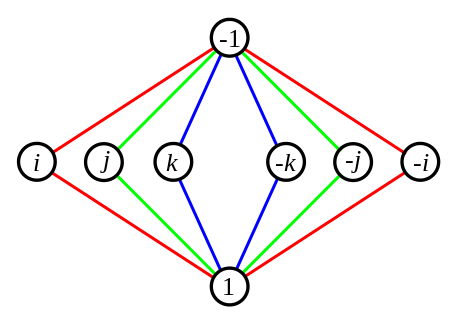
\includegraphics[width = .75\textwidth]{Figures/cycle.png}
\caption{Quaternions Cycle Diagram}
\label{fig:cycle}
\end{figure}
Despite being a non-abelian group, every subgroup of the group is normal subgroup.
This property is known as being \textit{Hamiltonian}.

\end{thm}

\subsection{Geometry \& Quaternions}
As discussed in Section \ref{sub:geo}, the primary methods of transformations that will be dicussed are translation and rotation.
When using quaternions for geometry, usually the \textit{Pure Quaternion} is used \cite{moderngeometries}.
A pure quaternion is simply a quaternion in the form of $\qq = x\qi + y\qj + z\qk$ because it can be used to represent a point in 3D.
We define a \textit{dot product} of two quaternions \qq$ $ and \qr$ $ by the following equation:
\begin{equation}
-S(\qq\qr) = x_1x_2 + y_1y_2 + z_1z_2.
\end{equation}
This is analagous to the traditional dot product $\qq \cdot \qr = \abs{\qq}\abs{\qr}cos(\phi)$, where $\phi$ is the angle between the vectors \qq$ $ and \qr$ $ in 3D.
Similarly, we can define a cross product bewteen \qq$ $ and \qr$ $ as the following:
\begin{equation}
V(\qq\qr) = (y_1z_2 - y_2z_1)\qi - (x_1z_2 - x_2z_1)\qj -(x_1y_2-x_2y_1)\qk.
\end{equation}
Again, this is the same as the geometric $\qq \times \qr = \abs{\qq}\abs{\qr}sin(\phi)\qu$, where $\phi$ is the same as before, and \qu$ $ is a pure unit quaternion and represents a unit vector perpedicular to the plane formed by \qq$ $ and \qr.
Figure \ref{fig:cross} shows the geometric representation of the cross product.

\begin{figure}[H]
\centering
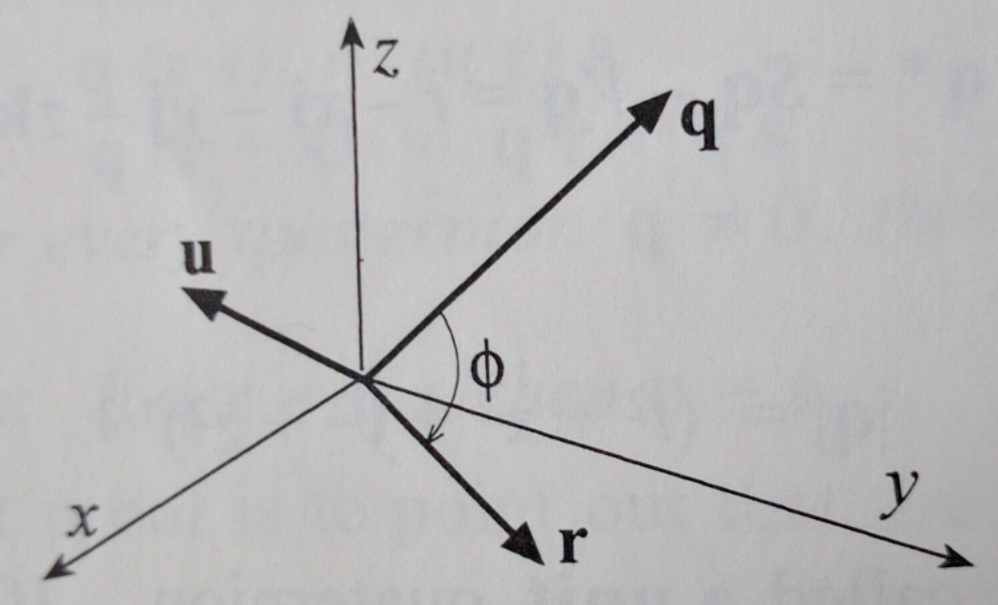
\includegraphics[width = .75\textwidth]{Figures/cross_product}
\caption{Visualizing $\qq \times \qr$}
\label{fig:cross}
\end{figure}

By combining the scalar result of the dot product and the vector result of the cross product, we can construct quaternion multiplication:
\begin{equation}
\label{eq:mult}
\qq\qr = -(\qq \cdot \qr) + (\qq \times \qr).
\end{equation}

This give us a geometric way of visualizing quaternion multiplication.
\\ \\
\noindent There is one more prerequisite before we can do rotations with quaternions.
Just like complex numbers can be represented in a polar form $z = \abs{z}(cos(\theta) + isin(\theta))$, we can express quaternions in a similar form of $\qq = \abs{\qq}(cos(\theta) + \qu sin(\theta))$.
Here, instead of the imaginary number $i$, we use the pure unit quaternion $\qu$.
Therefore, we have the following theorem:
\begin{thm}
Every quaternion can be represented in the form:
$$ \qq = \abs{\qq}(cos(\theta) + \qu sin(\theta))$$.
\end{thm}

With the above theorems and definitions, we are now able to represent rotation in 3D space with quaternions.

\begin{thm}
Let \qr$ $ be a unit quaternion. Let R be the transformation on the pure quaternion \qq$ $ defined by $$ \text{R}\qq = \qr \qq \qr^*.$$
Then, R is a rotation of the three dimensional space of pure quaternions about an axis passing through the origin.
If we take \qr$ $ in the polar form: $$ \qr = cos(\theta) + \qu sin(\theta), $$ where \qu$ $ is a unit quaternion, then R\qq$ $ is the pure quaternion obtained by rotating \qq$ $ about \qu$ $ by the angle $2\theta$.
Every rotation about an axis passing through the origin can be expressed this way.
\\ \\ \noindent \textit{Proof:} Let us look at R\qq$ $ for three cases, $\qq=\qu$, \qq$ $ is perpendicular to \qu$ $, and \qq$ $ is any pure quaternion.
\\ \\ Case 1: $\qq = \qu$
\\ Then $\text{R}\qu = \qr \qu \qr^* = (cos(\theta) + \qu sin(\theta)) \qu (cos(\theta) - \qu sin(\theta))$.
Expanding this yields $$ \text{R}\qu = cos(\theta)^2\qu - sin(\theta)^2 \qu^3 = cos(\theta)^2 \qu - sin(\theta)^2 (-\qu) = \qu.$$
Thus \qu$ $ is a fixed point of R.
This is expected because $\text{R}\qu$ is the rotation of \qu$ $ about the axis \qu.
\\ \\ Case 2: \qq$ $ is perpendicular to \qu.
\\ Then $\text{R}\qu = \qr \qq \qr^* = (cos(\theta) + \qu sin(\theta))\qq (cos(\theta) - \qu sin(\theta))$
\\ $ = cos(\theta)^2 \qq + \qu \qq cos(\theta)sin(\theta) - \qq \qu cos(\theta) sin(\theta) - \qu \qq \qu sin(\theta)^2.$
Using Equation \ref{eq:mult}, we get: $$ \qu \qq = -(\qu \cdot \qq) + (\qu \times \qq) = (\qu \times \qq),$$ because \qu$ $ and \qq$ $ are perpendicular.
Similarly, $$ \qq \qu = (\qq \times \qu) = -(\qu \times \qq)$$, so: $$ \qu \qq \qu = (\qu \cdot (\qu \times \qq)) - (\qu \times (\qu \times \qq)) = -(\qu \times(\qu \times \qq)).$$
Therefore $ \qu \qq \qu = \qq$.
When we put this all together we get $$ \text{R}\qq = cos(\theta)^2 \qq + 2 cos(\theta)sin(\theta)(\qu \times \qq) - sin(\theta)^2 \qq \\ = cos(2\theta)\qq + sin(2\theta)(\qu \times \qq).$$
Therefore, R\qq$ $ is the rotation of \qq$ $ through an angle of $2\theta$ about the axis of \qu.
\\ \\ Case 3: \qq$ $ is any pure quaternion.
First note that R is a linear transformation, that is, $R(\qq + \qr) = R(\qq) + R(\qr)$ and $R(\alpha\qq) = \alpha R(\qq)$.
Secondly notice that the rotation of 3D space is also a linear transformation.
To prove that two linear transformations are equal, it is enough to prove that they have the same effect on the vectors from some basis of 3D space.
We have shown that the rotation R and the rotation about the axis \qu$ $ by the angle $2\theta$ are equal when $\qu = \qq$ and \qu$ $ is perpendicular to \qu.
However, a basis for 3D space can be found consisting of the vector \qu$ $ plus two orthogonal vectors.
Therefore, R acts like a rotation for all 3D vectors. \qed

\end{thm}
